%% ****** Start of file aiptemplate.tex ****** %
%%
%%   This file is part of the files in the distribution of AIP substyles for REVTeX4.
%%   Version 4.1 of 9 October 2009.
%%
%
% This is a template for producing documents for use with 
% the REVTEX 4.1 document class and the AIP substyles.
% 
% Copy this file to another name and then work on that file.
% That way, you always have this original template file to use.

\documentclass[aip,amsmath,amssymb,reprint,twocolumn]{revtex4-1}
%\documentclass[aip,reprint]{revtex4-1}

\usepackage{graphicx,hyperref}
% \usepackage{pdfsync}

\newcommand{\relphantom}[1]{\phantom{\mathrel{#1}}}
\newcommand{\abs}[1]{\left|#1\right|}
\newcommand{\Nbasis}{{N_{\text{basis}}}}
\newcommand{\Nx}{{N_{x}}}
\DeclareMathOperator{\Real}{Re}
\DeclareMathOperator{\Imag}{Im}

\begin{document}

% Use the \preprint command to place your local institutional report number 
% on the title page in preprint mode.
% Multiple \preprint commands are allowed.
%\preprint{}

\title{The pseudo-spectral method, Gaussian quadrature and quasi-Gaussian quadrature: What Graham knows about the spectral method} %Title of paper

% repeat the \author .. \affiliation  etc. as needed
% \email, \thanks, \homepage, \altaffiliation all apply to the current author.
% Explanatory text should go in the []'s, 
% actual e-mail address or url should go in the {}'s for \email and \homepage.
% Please use the appropriate macro for the type of information

% \affiliation command applies to all authors since the last \affiliation command. 
% The \affiliation command should follow the other information.

\author{G.R. Dennis}
\email[]{graham.dennis@anu.edu.au}
%\homepage[]{Your web page}
%\thanks{}
%\altaffiliation{}


% Collaboration name, if desired (requires use of superscriptaddress option in \documentclass). 
% \noaffiliation is required (may also be used with the \author command).
%\collaboration{}
%\noaffiliation

\date{\today}

\begin{abstract}
% insert abstract here
This is a set of notes describing what Graham knows about the pseudo-spectral method.  I use this to obtain an approximate discrete Hankel transform appropriate for problems with Neumann boundary conditions.

\end{abstract}

\pacs{}% insert suggested PACS numbers in braces on next line

\maketitle %\maketitle must follow title, authors, abstract and \pacs

% Body of paper goes here. Use proper sectioning commands. 
% References should be done using the \cite, \ref, and \label commands
\section{Introduction}
\label{sec:Introduction}

In the spectral method, the idea is to approximate the exact solution $u(x)$ as a sum of $N$ orthonormal basis functions $\phi_i(x)$:
\begin{align}
  u(x) &\approx u_N(x) = \sum_i u_i \phi_i(x), \label{eq:BasisFunctionExpansion}
\end{align}
where $u_i$ are the expansion coefficients.  Often we need more than just the coefficients $\{u_i\}$, we also need the solution at the grid points.  Typically this is because we need to compute terms like $V(x) u(x)$ or $u(x)^2$.  We can always interpolate the solution onto a given set of coordinate points $\{x_i\}$ by using the expansion \eqref{eq:BasisFunctionExpansion}.  So in principle, we can choose the $\{x_i\}$ by any process and interpolate to compute $u_N(x_i)$.  The expression $V(x) u(x)$ can then be computed straight-forwardly at the grid points $x_i$.  If this term contributes to the evolution of $u(x)$, we now need the basis decomposition of $V(x) u(x)$, i.e.\ we need to invert our interpolation.  Now if $V(x) u(x)$ can be represented exactly in terms of the $N$ basis functions $\phi_i(x)$, then we can just invert our interpolation matrix to determine the basis function decomposition of $V(x) u(x)$.  Interpolation can be considered to be the application of the matrix $T_{ij}$ to the vector $u_j$:
\begin{align}
  u(x_i) &= \sum_j T_{ij} u_j,
\end{align}
where $T_{ij} = \phi_j(x_i)$.  This matrix can be inverted to find the $u_j$ from $u(x_i)$:
\begin{align}
  u_j &= \left(T^{-1}\right)_{ji} u(x_i).
\end{align}

However, in general $V(x) u(x)$ will be outside the span of the \emph{finite} set of basis functions $\{\phi_i(x)\}$.  In this case, applying the above procedure can lead to disastrous results.  For example, if $V(x) u(x)$ is a normalised basis function \emph{outside} the basis set $\{\phi_i(x)\}$ (i.e.\ we assume that the finite set $\{\phi_i(x)\}_{i=1}^N$ is the first $N$ terms of the complete, orthonormal set $\{\phi_i(x)\}_{i=1}^\infty$), then we can find that the $\sum_{i=1}^N \abs{u_i}^2$ can be much greater than 1.  We want $\sum_{i=1}^N \abs{u_i}^2 = \mathcal{O}(1)$ so that small amplitudes of higher-order basis functions don't pollute the other basis coefficients.

An alternative procedure would be to compute the basis coefficients of an arbitrary function $f(x)$ by exploiting the orthonormality of the basis functions:
\begin{align}
  f_i &= \int_a^b w(x) f(x) \phi_i(x)\, dx,
\end{align}
where $w(x)$ is a non-negative weight function (which is problem-dependent), and the $f_i$ are the basis coefficients.  This procedure will work well, but these integrals may not have analytic solutions, or $u(x)$ itself may not be known, we may only know $\{u(x_i)\}$.  In this case, we need to approximate the integral, for which we will use a quadrature formula of the form:
\begin{align}
  \int_a^b w(x) f(x) \, dx \approx \sum_{i=1}^N w_i f(x_i),
\end{align}
where the $\{w_i\}$ and $\{x_i\}$ are the weights and abscissas of the quadrature formula.  For a quadrature formula to be useful, we have the restrictions $w_i \ge 0$ and $x_i \in [a, b]$.

How should we choose the $w_i$ and $x_i$ in general?  Ideally we'd like our quadrature formula to preserve the orthonormality of our basis functions,
\begin{align}
  \int_a^b w(x) \phi_i(x) \phi_j(x)\, dx &\approx \sum_p w_p \phi_i(x_p) \phi_j(x_p) = \delta_{ij}, \label{eq:DiscreteOrthonormality}
\end{align}
where $\delta_{ij}$ is the Kronecker delta.  If we have $N$ basis functions and we (perhaps arbitrarily) decide to limit ourselves to $N$ abscissas $x_i$, we only have $2N$ degrees of freedom: $N$ weights $w_i$ and $N$ abscissas $x_i$.  But we have $1/2 (N^2 + N)$ orthonormality constraints to enforce (Equation~\eqref{eq:DiscreteOrthonormality} has $N^2$ terms, but the equation is symmetric exchanging $i$ and $j$).

In some situations, $\phi_i(x) \phi_j(x)$ can be expressed as a \emph{finite} sum of basis functions of order no higher than $2N$, in which case, choosing our $2N$ degrees of freedom to exactly integrate the first $2N$ basis functions ensures that the quadrature integrals of every pair of basis functions $f_i(x) f_j(x)$ are equal to their exact integrals.  This situation occurs when the $\phi_i(x)$ are polynomials with highest degree $i-1$ (any set of orthogonal polynomials satisfies this).  This situation also occurs for trigonometric series, for example $\cos(n \pi x) \cos(m \pi x)$ can be expressed in terms of $\cos[(m-n)\pi x]$ and $\cos[(m+n)\pi x]$.

Unfortunately, this is not always the case, a good example are the Bessel functions.  In this case our basis functions are $J_m(k_i x)$, but products of basis functions cannot be expressed as a \emph{finite} sum of other basis functions, i.e.\ $J_m(k_i x) J_m(k_j x)$ cannot be expressed as a finite sum of $J_m(k_i x)$.  In this case, we just need to do the best we can with our $2N$ degrees of freedom (or increase the number of abscissas $x_i$).  What we want is for the orthonormality matrix \eqref{eq:DiscreteOrthonormality} to be as close to the identity as possible.  To quantity this, we need an error norm.

Intuitively, we want all the eigenvalues of the orthonormality matrix to be as close to 1 as possible to ensure long-term stability of the solution after repeated application of interpolation and quadrature integration operations.  More specifically, we want the eigenvalues of the error matrix
\begin{align}
  \Delta_{ij} &= \sum_p w_p \phi_i(x_p) \phi_j(x_p) - \delta_{ij}
\end{align}
to have eigenvalues as small as possible.  We want to minimise something like:
\begin{align}
  E_1(\{w_p\}, \{x_p\}) &= \sum_i \abs{\lambda_i}^2.
\end{align}
It turns out that this is the Schatten $p$-norm of $\Delta_{ij}$ with $p=1$.  This is not particularly convenient because to efficiently minimise any error norm we will need to be able to compute its derivatives with respect to the weights $\{w_p\}$ and abscissas $\{x_p\}$, and computing the derivatives of the eigenvalues with respect to the entries of the matrix is troublesome and can be numerically unstable.  A numerically more convenient norm is the $p=2$ Schatten $p$-norm, which is also the Frobenius norm:
\begin{align}
  E_2(\{w_p\}, \{x_p\}) &= \sqrt{ \sum_i \abs{\lambda_i}^4} = \sqrt{\sum_{ij} \abs{\Delta_{ij}}^2}.
\end{align}
The latter expression is simple to evaluate \emph{and} simple to find an expression for the derivatives of the error.  The python code \verb+playground.py+ uses the square of this error norm because it simplifies the expressions for the derivatives.

Often the discrete basis function decomposition is related to an integral transform (e.g.\ the Fourier transform, Hankel transform, etc.).  In this case, we would like to have results like Parseval's theorem for our discretised transforms.  For example, if $\alpha_i \phi_i(x) =  \psi_{k_i}(x)$ for some $k_i$ and where $\alpha_i$ is a positive real normalisation constant, we may have the integral transform
\begin{align}
  \tilde{f}(k) &= \int w(x) f(x) \psi^*_k(x)\, dx, \label{eq:IntegralTransform}
\end{align}
for which we would like to preserve a result like Parseval's theorem\footnote{Parseval's theorem reduces to Plancheral's theorem $\int w(x) |f(x)|^2\, dx = \int w(k) |\tilde{f}(k)|^2\, dk$ for $g(x)$ equal to $f(x)$.}, i.e.
\begin{align}
  \int w(x) f^*(x) g(x)\, dx &= \int \tilde{w}(k) \tilde{f}^*(k) \tilde{g}(k)\, dk.
\end{align}

From equation~\eqref{eq:IntegralTransform}, we can relate $\tilde{f}(k)$ to the basis coefficients $f_i$,
\begin{align}
  \tilde{f}(k_i) &= \int w(x) \sum_j f_j \phi_j(x) \psi_{k_i}^*(x) \, dx \\
  &= \int w(x) \sum_j f_j \phi_j \alpha_i \phi_i^*(x)\, dx = \alpha_i f_i.
\end{align}
Note that no approximations have been made at this point (although we have assumed we know the basis expansion $\{f_i\}$ of $f(x)$).  Computing the left hand side of Parseval's theorem gives
\begin{align}
  \int w(x) f^*(x) g(x)\, dx &= \int w(x) \sum_{ij} f_i^* g_j \phi_i^*(x) \phi_j(x)\, dx\\
   &= \sum_i f_i^* g_i = \sum_i \frac{1}{\alpha_i^2} \tilde{f}^*(k_i) \tilde{g}(k_i).
\end{align}
Thus if we use the quadrature formula
\begin{align}
  \int \tilde{w}(k) \tilde{f}(k) \, dk &\equiv \sum_i \frac{1}{\alpha_i^2} \tilde{f}(k_i),
\end{align}
to evaluate the integral on the right-hand side of Parseval's theorem, then Parseval's theorem will apply to our discrete transform.  Although no approximations have been made in `proving' Parseval's theorem for the discretised integral transform, performing the integral on the left-hand side of Parseval's theorem will in practice be done by means of the quadrature integral
\begin{align}
  \int w(x) f^*(x) g(x)\, dx &\approx \sum_i w_i f^*(x_i) g(x_i),
\end{align}
and so the degree to which Parseval's theorem will hold will be determined by the quality of the quadrature integral, and hence by the magnitude of the error norm mentioned earlier, which we wish to minimise.

\section{Statement of the method}
\label{sec:Method}

Consider the general case of $\Nbasis$ (possibly complex) basis functions $\{\phi_i(x)\}_{i=1}^{\Nbasis}$ (which are the first $\Nbasis$ elements of the complete, orthonormal set $\{\phi_i(x)\}_{i=1}^{\infty}$) and $\Nx$ spatial points in our grid.  In this case we want to minimise the error norm
\begin{align}
  \Gamma &= E_2^2\left(\{w_p\}, \{x_p\}\right) = \sum_{ij} \abs{\Delta_{ij}}^2, \label{eq:TransformError}
\end{align}
where
\begin{align}
  \Delta_{ij} &= \sum_{p} w_p \phi_i^*(x_p) \phi_j(x_p) - \delta_{ij},
\end{align}
is the error matrix.  The partial derivatives of $\Gamma$ with respect to the weights and abscissas are
\begin{align}
  \frac{\partial \Gamma}{\partial w_p} &= 2 \sum_{ij}\Real\left\{\Delta_{ij}^* \phi_i^*(x_p) \phi_j(x_p)\right\}, \label{eq:ErrorWeightDerivative}\\
  \frac{\partial \Gamma}{\partial x_p} &= 2 \sum_{ij}\Real\left\{\Delta_{ij}^* w_p \left[{\phi_i'}^*(x_p) \phi_j(x_p) + \phi_i^*(x_p) \phi_j'(x_p)\right] \right\} \notag\\
   &= 4 \sum_{ij}\Real\left\{\Delta_{ij}^* w_p \phi_i^*(x_p) \phi_j'(x_p)\right\}. \label{eq:ErrorAbscissaDerivative}
\end{align}

Given $\Nbasis$ basis functions (and their derivatives) and an initial guess for the $\Nx$ weights $\{w_p\}$ and $\Nx$ abscissas $\{x_p\}$ we can now efficiently minimise $\Gamma$ numerically using the derivatives given by Eqs.~\eqref{eq:ErrorWeightDerivative} and \eqref{eq:ErrorAbscissaDerivative}.  This minimisation procedure is implemented in \verb+playground.py+.

In practice, we may choose $\Nx$ given $\Nbasis$ (or \emph{vice versa}) to ensure that the minimum value of $\Gamma$ is sufficiently small.

We want to apply this method to the Hankel transform, for which no quadrature formula with $\Nx < \frac{1}{4}(\Nbasis^2 + \Nbasis)$ spatial grid points can be exact.  Ideally we would like $\Nx \sim \mathcal{O}(\Nbasis)$.

\section{The Hankel transform}

One of the useful properties of the Hankel transform is that it provides accurate computation of the Laplacian for problems with radial symmetry:
\begin{align}
  \nabla^2 \left[f(r) e^{i m \theta}\right] &= \left\{\mathcal{H}^{-1}_m\left[(-k^2)\tilde{f}(k)\right](r)\right\}e^{i m \theta}
\end{align}
where the $m$-order Hankel transform and its inverse are defined by
\begin{align}
  \mathcal{H}_m[f](k) &= \tilde{f}(k) = \int_0^{\infty} r f(r) J_m(k r) \, dr \label{eq:HankelTransform}\\
  \mathcal{H}^{-1}_m[\tilde{f}](r) &= f(r) = \int_0^{\infty} k \tilde{f}(k) J_m(k r)\, dk, \label{eq:InverseHankelTransform} 
\end{align}
where $J_m(r)$ is the Bessel function of the first kind of order $m$. Or improve the notation as appropriate.  I've never actually seen the $\mathcal{H}_m$, $\mathcal{H}^{-1}_m$ notation used anywhere.

The motivation of the discrete Hankel transform is to get a similar property on finite domains.  If we expand our function $f(r)$ in terms of a sum of Bessel functions
\begin{align}
  f(r) &= \sum_i \frac{f_i}{\alpha_i} J_m(k_i r), \label{eq:DiniSeries}
\end{align}
where the $\alpha_i$ are positive real normalisation constants defined by
\begin{align}
  \int_0^R r J_m^2(k_i r)\, dr &= \alpha_i^2, \label{eq:AlphaNormalisation}
\end{align}
then the Laplacian is easy to calculate
\begin{align}
  \nabla^2\left[f(r) e^{i m \theta}\right] &= \sum_i \frac{f_i}{\alpha_i} \nabla^2\left[J_m(k_i r) e^{i m \theta}\right] \\
  &= \sum_i - k_i^2 \frac{f_i}{\alpha_i} J_m(k_i r) e^{i m \theta}.
\end{align}
Note that the $k_i$ are chosen such that $f(r)$ satisfies an homogenous boundary condition at $r=R$, i.e.\ a boundary condition of the form $a f(R) + b f'(R) = 0$.  This ensures that the basis functions are complete and orthogonal (Eq.~\eqref{eq:DiniSeries} is a Dini series\citep{Watson:1966}).

The coefficients $f_i$ can be determined from $f(r)$ by performing the Hankel transform, Eq.~\eqref{eq:HankelTransform}.  However, that requires an integral over the infinite domain $[0, \infty)$, which is problematic as we want to deal with the finite domain $[0, R)$.  To solve this, we can define the function $f_R(r) \equiv f(r) \Pi_R(r)$, where $\Pi_R(r)$ is the top-hat function which is 1 for $r < R$ and zero for $r > R$.  The Hankel transform of $f_R(r)$ can be conveniently be computed in terms of an integral over the finite domain $[0, R)$,
\begin{align}
  \tilde{f}_R(k) &= \int_0^\infty r f_R(r) J_m(k r)\, dr = \int_0^R r f(r) J_m(k r)\, dr.
\end{align}
The $f_i$ can be obtained from $\tilde{f}_R(k)$ using
\begin{align}
  \tilde{f}_R(k_i) &= \int_0^R r \sum_j \frac{f_j}{\alpha_j} J_m(k_j r) J_m(k_i r)\, dr = \alpha_i f_i,
\end{align}
where we have used the orthogonality of the $J_m(k_i r)$.

On the restricted domain $[0, R)$ we thus have the \emph{exact} Hankel transform pair
\begin{align}
  \tilde{f}_R(k_i) &= \int_0^R r f(r) J_m(k_i r)\, dr, \label{eq:FiniteHankelTransform}\\
  f(r) &= \sum_i \frac{1}{\alpha_i^2} \tilde{f}_R(k_i) J_m(k_i r). \label{eq:FiniteInverseHankelTransform}
\end{align}
In order to work with this transform pair computationally, we need to approximate the integral in Eq.~\eqref{eq:FiniteHankelTransform} with a quadrature formula.  Once we do this, we have the discrete Hankel transform (or quasi-discrete Hankel transform).

\subsection{(Quasi-)discrete Hankel transform}

Most derivations of the quasi-discrete Hankel transform start with the continuous Hankel transform pair Eqs.~\eqref{eq:HankelTransform} and \eqref{eq:InverseHankelTransform}, and then assume \emph{a priori} that the function $f(r)$ is non-zero only in the region $[0, R)$, and the corresponding $\tilde{f}(k)$ is non-zero only in the region $[0, K)$ for some constant $K$.  It is not usually stated as such, but this is an \emph{approximation}.  Any function (apart from the zero function) which is zero over the domain $[0, R)$ will have a transform $\tilde{f}(k)$ which is non-zero for arbitrarily large $k$ (but it does decay).

Our derivation will begin with the exact `restricted' Hankel transform pair, Eqs.~\eqref{eq:FiniteHankelTransform} and \eqref{eq:FiniteInverseHankelTransform}.  Although $\tilde{f}_R(k)$ is only evaluated at the $k_i$ in \eqref{eq:FiniteInverseHankelTransform}, it is defined for all $k$,
\begin{align}
  \tilde{f}_R(k) &= \sum_i \tilde{f}_R(k_i) C(k; k_i),
\end{align}
where $C(k; k_i)$ is defined by
\begin{multline}
C(k; k_i) = \frac{1}{\alpha_i^2}\frac{R}{k_i^2 - k^2} \Big[k J_m(k_i R) J_m'(k R) \\ - k_i J_m(k R) J_m'(k_i R) \Big], \label{eq:CardinalFunction}
\end{multline}
which is a `cardinal' function (see \citet{Whittaker:1914}; \citet[Chapter 5]{SpectralMethods}; or in the context of Bessel functions, \citet{Rawn:1989}) which satisfies
\begin{align}
  C(k_j; k_i) &= \delta_{ij}.
\end{align}
In other words, $C(k; k_i)$ takes the value 1 at $k=k_i$, and is zero for $k = k_j$ for $i \neq j$.  A relevant property of the $C(k; k_i)$ functions is that they are largest when $k$ is close to $k_i$, but decay as $k$ grows large, see Figure~\ref{fig:CardinalFunctions}.

\begin{figure}
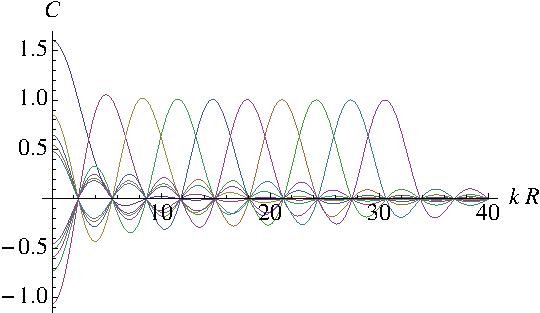
\includegraphics[width=8cm]{First10DirichletCardinalFunctions}
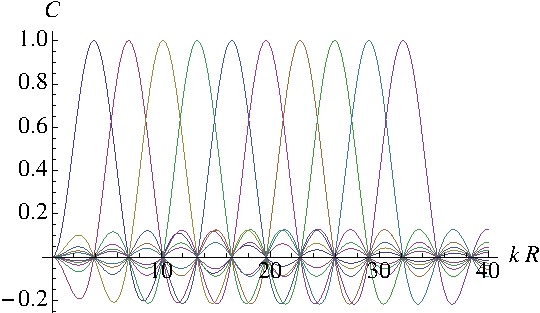
\includegraphics[width=8cm]{First10NeumannCardinalFunctions}
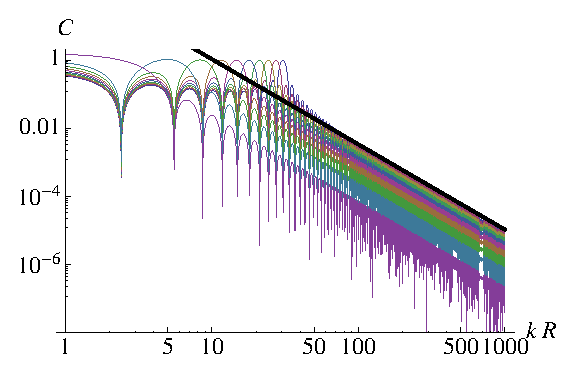
\includegraphics[width=8cm]{First10DirichletCardinalFunctionsScaling}
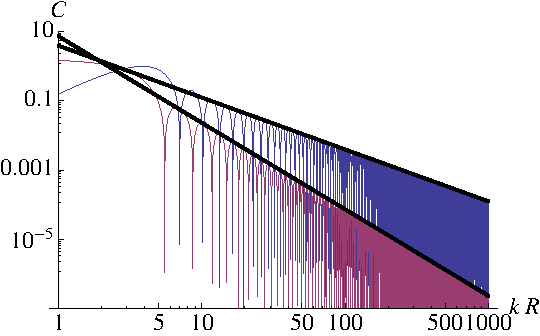
\includegraphics[width=8cm]{CardinalFunctionDirichletVsNeumannScaling}
\caption{(a) First 10 Cardinal functions for Dirichlet boundary conditions ($f(R) = 0 \implies J_m(k_i R) = 0$); (b) First 10 Cardinal functions for Neumann boundary conditions ($f'(R) = 0 \implies J_m'(k_i R) = 0$); (c) Asymptotic scaling of the first 10 Cardinal functions for Dirichlet boundary conditions and a comparison to the asymptotic $k^{-5/2}$ scaling; (d) Comparison of the asymptotic scaling of the first Cardinal functions for Dirichlet (reddish) and Neumann (blue) boundary conditions comparing the $k^{-5/2}$ and $k^{-3/2}$ scaling respectively.\label{fig:CardinalFunctions}}
\end{figure}

To fully discretise the `restricted' transform, Eqs.~\eqref{eq:FiniteHankelTransform} and \eqref{eq:FiniteInverseHankelTransform}, we must choose a quadrature formula to evaluate the integral in Eq.~\eqref{eq:FiniteHankelTransform}.  In this, we are motivated by the identity
\begin{align}
  f(r) &= \int_0^\infty k \tilde{f}_R(k) J_m(k r)\, dk = \sum_i \frac{1}{\alpha_i^2} \tilde{f}_R(k_i)J_m(k_i r),
\end{align}
which is true for $r \in [0, R)$.  A similar identity can be obtained for integrals over $r$:
\begin{align}
  \int_0^\infty r g_K(r) J_m(k r)\, dr &= \sum_i \frac{1}{\beta_i^2} g_K(r_i) J_m(k r_i), \label{eq:CoordinateIntegral}
\end{align}
where $\tilde{g}(k)$ is defined by
\begin{align}
  \tilde{g}(k) &= \sum_i \frac{\tilde{g}_i}{\beta_i} J_m(k r_i), \label{eq:DiniSeriesInK}
\end{align}
the function $\tilde{g}_K(k)$ is defined similarly to $f_R(r)$ as $\tilde{g}_K(k) = g(k) \Pi_K(k)$, which is zero for $k > K$, and the $r_i$ are chosen so that $g(k)$ satisfies an homogenous boundary condition at $k=K$.  

The identity Eq.~\eqref{eq:CoordinateIntegral} applies to integrals over the range $(0, \infty)$, however we need an approximation for integrals over the range $(0, R)$.  If we replace $g_K(r)$ with $f_R(r)$, then we would obtain
\begin{align}
  \int_0^R r f_R(r) J_m(k r)\, dr &\approx \sum_i \frac{1}{\beta_i^2} f_R(r_i) J_m(k r_i),  \label{eq:ApproximateQuadrature}
\end{align}
which is a quadrature approximation of the form we desire, however, the identity Eq.~\eqref{eq:CoordinateIntegral} is only valid for functions which have a Hankel transform that is zero for $k > K$, and this is not exactly true for $f_R(r)$.  The cardinal functions $C(k; k_i)$ that comprise $\tilde{f}_R(k)$ are not zero above some $K$, however they do decay (see Figure~\ref{fig:CardinalFunctions}) for $k > k_i$.  Thus the quadrature rule \eqref{eq:ApproximateQuadrature} is approximate and its error will be determined by the asymptotic scaling of the cardinal functions as $k\rightarrow\infty$ (this error is analysed in detail in Section~\ref{sec:ErrorAnalysis}).  In the case of Dirichlet boundary conditions for $f(r)$ (i.e.\ $f(R) = 0$), the first term in brackets in Eq.~\eqref{eq:CardinalFunction} is zero (as $J_m(k_i R) = 0$), and the cardinal functions scale asymptotically as $k^{-5/2}$.  For all other boundary conditions, the first term in Eq.~\eqref{eq:CardinalFunction} will be non-zero and will dominate the asymptotic scaling, and the cardinal functions will decay as $k^{-3/2}$ (see Figure~\ref{fig:CardinalFunctions}).  

The fundamental reason for the different asymptotic scalings of $\tilde{f}_R(k)$ for different boundary conditions is that $f_R(r)$ has a discontinuous derivative at $r=R$ if it obeys Dirichlet boundary conditions, however for all other boundary conditions $f_R(r)$ itself is discontinuous at $r=R$.  For Fourier transforms, if a function is continuous and its first $k$ derivatives are continuous, then the Fourier series coefficients will decay as $a_n \sim O(n^{-k})$.  A similar property will likely hold for the Hankel transform, and the cardinal functions are Hankel transforms of Bessel functions multiplied by the top-hat function\footnote{This paragraph makes no sense, does it?}.  If the Bessel functions obey Dirichlet boundary conditions at $r=R$, then only the derivative of the function will be discontinuous, however if other homogenous boundary conditions are instead satisfied, then the function itself will be discontinuous and we may expect its Hankel transform to decay more slowly.

Now that we have chosen the quadrature formula, Eq.~\eqref{eq:ApproximateQuadrature}, to approximate the integral in Eq.~\eqref{eq:FiniteHankelTransform}, all that remains is to choose $K$ and a boundary condition for $\tilde{g}(k)$ at $k=K$ to determine the abscissas $r_i$.  Given that $\tilde{g}(k)$ is an approximation to $\tilde{f}_R(k)$, which is a weighted sum of cardinal functions $C(k; k_i)$ which are zero for $k=k_j$ where $i \neq j$, a good choice for $K$ and the boundary condition is $\tilde{g}(K)=0$ for some $K=k_{N_K}$ (other choices are possible, for example the Neumann boundary condition $\tilde{g}'(K)= 0$ was considered by \citep{Kai-Ming:2009}, however as we show in Section~\ref{sec:ErrorAnalysis}, this choice has a higher error than the Dirichlet condition described here).  The integer $N_K$ must be greater than $\Nbasis$ to ensure that all of the $\Nbasis$ cardinal functions are zero at $k=K$, and it must also be greater than $\Nx$ to ensure that all of the $r_i$ are less than $R$.  Thus a good choice for $N_K$ is $N_K = \max(\Nbasis,\Nx)+1$.  Typically $\Nx \ge \Nbasis$, and in this case $N_K = \Nx+1$.

We are now in a position to give the general form of the approximate discrete Hankel transform pair
\begin{align}
  \tilde{f}_R(k_i) &\approx \sum_{j=1}^{\Nx} \frac{1}{\beta_j^2} f_R(r_j) J_m(k_i r_j), \label{eq:GeneralDiscreteHankelTransform}\\
  f_R(r_i) &\approx \sum_{j=1}^{\Nbasis} \frac{1}{\alpha_j^2} \tilde{f}_R(k_j) J_m(k_j r_i), \label{eq:GeneralDiscreteInverseHankelTransform}\\
  \intertext{where}
  \alpha_i^2 &= \frac{R^2}{2} \left[\left(1 - \frac{m^2}{k_i^2 R^2}\right) J_m^2(k_i R) + J_m'^2(k_i R)\right], \label{eq:GeneralAlpha}\\
  \beta_i^2 &= \frac{K^2}{2} \left[\left(1 - \frac{m^2}{K^2 r_i^2}\right) J_m^2(K r_i) + J_m'^2(K r_i)\right], \label{eq:GeneralBeta}
\end{align}
where the $k_i$ are the first $\Nbasis$ roots of $a J_m(k_i R) + b k_i J_m'(k_i R) = 0$, and the $r_i$ are the first $\Nx$ roots of $c J_m(K r_i) + d r_i J_m(K r_i) = 0$, for some $a$, $b$, $c$, $d$, which define the homogenous boundary conditions obeyed by $f(r)$ at $r=R$ and $\tilde{f}(k)$ at $k = K$ respectively.  We give explicit expressions for two most common cases of Dirichlet boundary conditions for both $f(r)$ and $\tilde{f}(k)$ and Neumann boundary conditions for $f(r)$ and Dirichlet conditions for $\tilde{f}(k)$ (as in the case of a problem requiring Neumann conditions at $r=R$, but not specifying boundary conditions for $\tilde{f}(k)$, Dirichlet conditions will give an approximate transform with a lower error).

\subsubsection{Example 1: $f(R)=0$ and $\tilde{f}(K)=0$}
\label{sec:BoundaryConditionsDirichletDirichlet}

\begin{align}
  \tilde{f}_R(k_p) &\approx \frac{2 R^2}{S^2} \sum_{q=1}^{\Nx} \frac{1}{J_{m+1}^2(j_{m,q})} f_R(r_q) J_m\left(\frac{j_{m,p} j_{m,q}}{S}\right),\\
  f_R(r_p) &\approx \frac{2}{R^2} \sum_{q=1}^{\Nbasis} \frac{1}{J_{m+1}^2(j_{m,q})} \tilde{f}_R(k_q) J_m\left(\frac{j_{m,p} j_{m,q}}{S}\right),
\end{align}
where $k_i = j_{m,i}/R$, $r_i = R j_{m,i}/S$, $K = S/R$, and $S = j_{m, \Nx+1}$ with $j_{m,i}$ the $i$\textsuperscript{th} positive zero of the Bessel function $J_m(x)$.  We have also used the identity $J_{m}'(j_{m,q}) = -J_{m+1}(j_{m,q})$.

\begin{widetext}
\subsubsection{Example 2: $f'(R)=0$ and $\tilde{f}(K)=0$}
\label{sec:BoundaryConditionsNeumannDirichlet}

\begin{align}
  \tilde{f}_R(k_p) &\approx \frac{2 R^2}{S^2} \sum_{q=1}^{\Nx} \left[\left(1 - \frac{m^2}{{j'_{m,q}}^2}\right) J_m^2(j'_{m,q})\right]^{-1} f_R(r_q) J_m\left(\frac{j'_{m,p}j_{m,q}}{S} \right),\\
  f_R(r_p) &\approx \frac{2}{R^2} \sum_{q=1}^{\Nbasis} \frac{1}{J_{m+1}^2(j_{m,q})} \tilde{f}_R(k_q) J_m\left(\frac{j'_{m,q} j_{m,p}}{S}\right),
\end{align}
where $k_i = j'_{m,i}/R$, $r_i = R j_{m,i}/S$, $K = S/R$, and $S \approx j'_{m, \Nx+1}$ with $j_{m,i}$ the $i$\textsuperscript{th} positive zero of the Bessel function $J_m(x)$, and $j'_{m,i}$ the $i$\textsuperscript{th} positive zero of $J'_{m}(x)$, except that $x=0$ is considered to be the first zero of $J_0'(x)$ (see Chapter~18 of \citet{Watson:1966}).  Note that the value given for $S$ is approximate and the error of the approximate transform may be improved slightly by numerical optimisation, or as we will see in Section~\ref{sec:ErrorAnalysis}, more significantly by employing the approach described in Section~\ref{sec:Method}.

\end{widetext}

\subsection{Optimised quadrature for the Hankel transform}
\label{sec:OptimisedQuadrature}

The need to specify a boundary condition for $\tilde{g}(k)$ is an artefact of the method used to construct a quadrature rule to approximate the integral in the finite-domain Hankel transform, Eq.~\eqref{eq:FiniteHankelTransform}.  For that \emph{exact} Hankel transform pair, Eqs.~\eqref{eq:FiniteHankelTransform} and \eqref{eq:FiniteInverseHankelTransform}, boundary conditions only need to be specified for $f(r)$ at $r=R$.  We would therefore prefer to simply choose an optimum quadrature a given boundary condition and truncation $(\Nbasis, \Nx)$.  We will use the procedure described in Section~\ref{sec:Method} to optimise the quadrature rule.  The error properties of this rule will be examined in Section~\ref{sec:ErrorAnalysis}.

\subsection{History of the discrete Hankel transform}

The first record of the idea of the quasi-discrete Hankel transform (QDHT) seems to be \citet{Johnson:1987}, where he focussed exclusively on the Dirichlet boundary conditions.  \citet{Lemoine:1994} appears to have independently rederived it, and briefly discusses a transform with Neumann boundary conditions, mostly in response to the announcement of the work of \citet{Stade:1995}.  \citet{Stade:1995} focus on a transform with Neumann boundary conditions in coordinate space and Dirichlet boundary conditions in k-space (FIXME: verify this).  \citet{Yu:1998} seems to have independently derived the QDHT again as there is no citation for anything preceding it.  \citet{Yu:1998} considered the $m=0$ order case only, and that was generalised by \citet{Guizar-Sicairos:2004}, but that case had already been solved by \citet{Johnson:1987,Lemoine:1994}.  More recently, \citet{Kai-Ming:2009} have derived a transform assuming Neumann boundary conditions in both coordinate space and k-space.

Note most of the above methods derive transforms which have an undetermined quantity $S$, which is variously chosen to make the determinant of the (normalised) transform matrix unity, or to make the $\phi_{N+1}(x)$ basis function (the first basis function outside the finite basis set) be orthogonal with the first $N$ functions (according to the quadrature formula).

For the case of the Dirichlet boundary conditions there exists an analytic expression which is a good choice for $S$, in that it appears to be very close to optimal. Specifically the error norm described in section~\ref{sec:Introduction} is basically minimised as a function of $S$, and perturbing the $\{w_i\}$ and $\{x_i\}$ from this quadrature appears to yield very little benefit.

On the other hand, the existing schemes for Hankel transforms with Neumann boundary conditions have significantly larger errors which will be noticeable if you apply the transform and its inverse many times.  Using the scheme sketched in the previous section yields significant improvement over previous proposals.  Importantly, the optimisation can be performed relatively quickly on modern hardware.  For an $N=100$ quasi-discrete Hankel transform, the quadrature formula can be optimised in $\sim 75\text{s}$.  Importantly, the results of this optimisation procedure can be saved and re-used for subsequent simulations.

The methods presented here can be applied to the Dirichlet case, but with little benefit.  I don't understand why this is, but as we are able to substantially improve the Neumann case, that may be enough.



\section{Error analysis}
\label{sec:ErrorAnalysis}

Figure~\ref{fig:ErrorScaling} demonstrates that the (quasi-)discrete Hankel transform for Dirichlet boundary conditions has superior error scaling to the transform for Neumann boundary conditions.  Figure~\ref{fig:TransformErrorScaling} shows the improvement in the transform error $\Gamma$ by using the optimised quadrature described in Section~\ref{sec:OptimisedQuadrature}.  The improvement in $\Gamma$ is about 1-3 orders of magnitude for the Dirichlet transform (this would correspond to a uniform reduction in the eigenvalues of the error matrix $\Delta_{ij}$ of a factor of 2-6), however the improvement for the Neumann transform is much more significant of 7-9 orders of magnitude (which corresponds to a uniform reduction of the eigenvalues of the error matrix of $\Delta_{ij}$ of a factor of 50-200).  At the end of the day, it is the eigenvalues of $\Delta_{ij}$ that we wish to reduce, and a reduction of the eigenvalues by a factor of 10 means that we can perform approximately 10 times more transforms (in the process of, for example, numerical integration of a system of PDEs) before being limited by the transform error.

At this point it might be good to look at the eigenvalues of $\Delta_{ij}$ for a couple of cases and state the number of transforms that you could do before the accumulated error reached, say, a level of 1\%.

\begin{figure}
  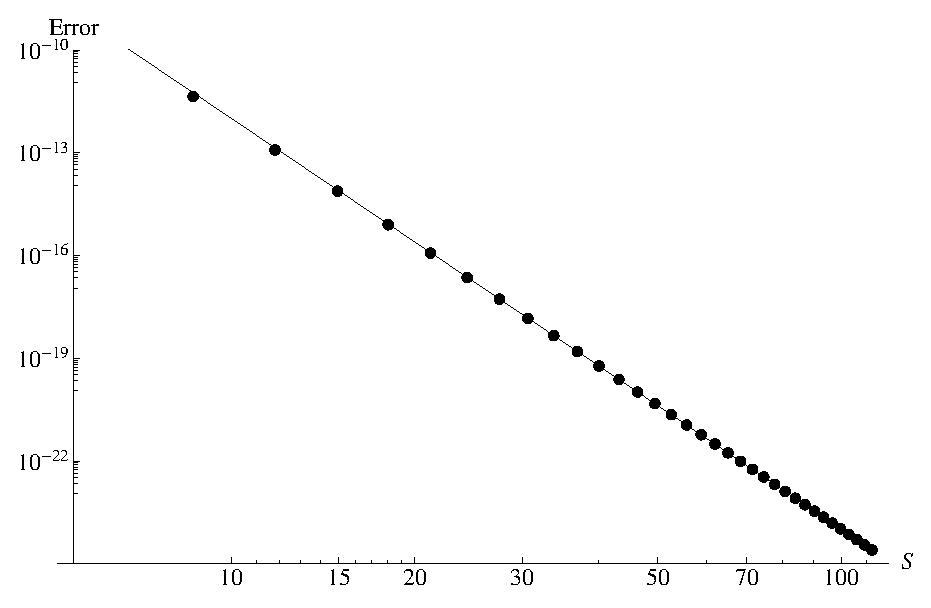
\includegraphics[width=8cm]{BesselDirichletErrorScaling}
  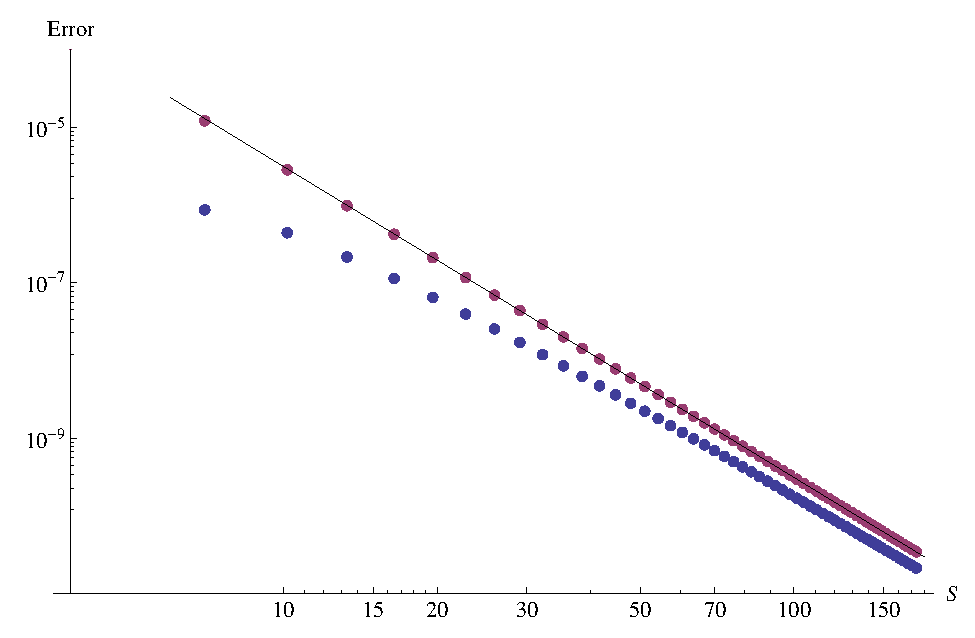
\includegraphics[width=8cm]{BesselNeumannErrorScaling}
  \caption{Plots of the square relative error in the quadrature integral of $\abs{\phi_1(r)}^2$ as a function of $\Nx$ for different $m=0$ discrete Hankel transforms, but plotted as a function of $S(\Nx)$ to better demonstrate asymptotic scaling.  Note that $S \propto \Nx$ as $\Nx \rightarrow \infty$. (a) Error of transform defined by Dirichlet--Dirichlet boundary conditions (see Section~\ref{sec:BoundaryConditionsDirichletDirichlet}), the error scales as $\mathcal{O}(S^{-12})$ (straight line of best fit is black solid line).  (b) Error of transform defined by Neumann--Dirichlet boundary conditions (see Section~\ref{sec:BoundaryConditionsNeumannDirichlet}), the error scales as $\mathcal{O}(S^{-4})$ (straight line of best fit is solid black line).  The purple dots correspond to the choice $S=j'_{0,\Nx+1}$, while the lower blue dots is the error obtained by choosing $S$ to minimise the error norm $\Gamma$ (see Eq.~\eqref{eq:TransformError}).  For $\Nx \lesssim 5$, this yields an error reduction of between a factor of 3 and 10, but for $\Nx \gtrsim 20$ the improvement is less than a factor of two, and reduces as $\Nx \rightarrow \infty$.\label{fig:ErrorScaling}}
\end{figure}

\begin{figure}
  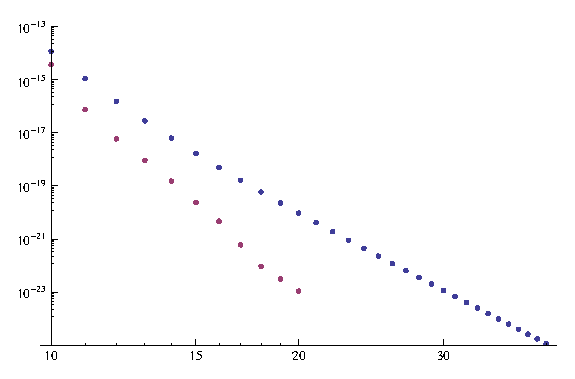
\includegraphics[width=8cm]{BesselDirichletMatrixNormErrorScaling}
  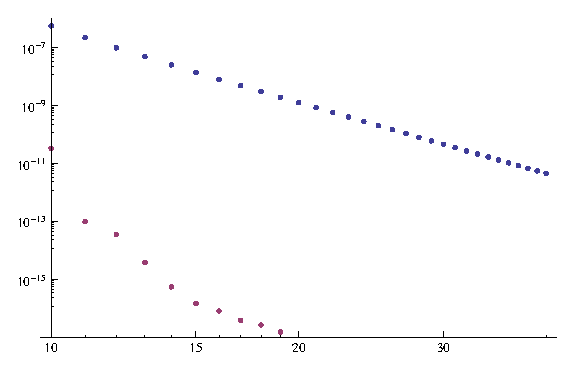
\includegraphics[width=8cm]{BesselNeumannMatrixNormErrorScaling}
  \caption{Plots of the transform error $\Gamma$ (see Eq.~\eqref{eq:TransformError}) for different $m=0$ discrete Hankel transforms for $\Nbasis=10$, as a function of $\Nx$.  (a) Dirichlet boundary conditions for $f(r)$, and (b) Neumann boundary conditions for $f(r)$.  In both plots the blue dots are the `standard' (quasi-)discrete Hankel transform described in Sections~\ref{sec:BoundaryConditionsDirichletDirichlet} [Figure (a)] or \ref{sec:BoundaryConditionsNeumannDirichlet} [Figure (b)], and the purple dots are the numerically optimised quadrature (see Section~\ref{sec:OptimisedQuadrature}). \label{fig:TransformErrorScaling}}
\end{figure}


\section{Example calculation}
\label{sec:Example}
Ideas for example: wave equation (should be similar to shallow water waves in a bucket); radial heat propagation in an isolated disk; whatever problem David Zwicker is solving.

\section{Conclusion}
\label{sec:Conclusion}

If you don't care about your boundary condition for the Hankel transform, use the (quasi-)discrete Hankel transform and don't bother with the numerical optimisation procedure.  The standard transform is almost always accurate enough, or you can always just increase $\Nbasis$ and/or $\Nx$ to significantly improve the error.  If you do care about your boundary condition, and you require Neumann (or another non-Dirichlet boundary condition) at $r=R$, then numerical optimisation of the quadrature rule can significantly reduce the transform error.

The quadrature optimisation procedure described in this paper is general to any problem for which we would like to use the spectral method with a particular set of (orthogonal) basis functions, but for which an exact Gaussian quadrature rule does not exist.  Other potential applications include solving problems on a circular disc \emph{without} any assumptions of angular symmetry.  In this case, the basis functions are $J_m(k_{m,i} r) e^{i m \theta}$, however no optimal quadrature exists.  As we have shown in this paper, for each $m$ a good choice exists for the abscissas $r_i$, but for different values of $m$, the optimal abscissas will be different.  Finding the optimal quadrature for the this problem could be done using the procedure described in this paper.


\bibliography{HankelNeumann.bib}


\end{document}
%
% ****** End of file aiptemplate.tex ******
